% Type de document :
\documentclass{rapportDeProjetENSICAEN}
\type{Rapport de projet}


% Caractéristiques du document :
\newcommand{\Nom}{Pellet}
\newcommand{\Prenom}{Eglantine}
\newcommand{\lastName}{Le Bécachel}
\newcommand{\firstName}{Pierre}
\newcommand{\Promotion}{Promotion 2017}
\newcommand{\Specialite}{Informatique}
\newcommand{\Majeure}{Majeure MSI}
\newcommand{\AnneeEnCours}{2017}
\newcommand{\AnneeUniversitaire}{Année 2016 - 2017}
\newcommand{\TuteurEntreprise}{Tuteur entreprise: Léonard Dallot}
\newcommand{\TuteurEcole}{Tuteur école: Patrick Lacharme}
\nomEntreprise{One Wave}
\adresseEntreprise{Incubateur de Telecom Bretagne, 2 rue de la Chataîgneraie 35510 Cesson-Sévigné}
\newcommand{\TitrePrincipal}{Rapport de projet 3ème année}
\newcommand{\SousTitre}{"Transport d'informations contextuelles au sein d'une transaction EMV"}
\promotion{\Promotion}
\specialite{\Specialite}
\majeure{\Majeure}
\anneeEnCours{\AnneeEnCours}
\anneeUniversitaire{\AnneeUniversitaire}
\nom{\Nom}
\prenom{\Prenom}
\lastName{\lastName}
\firstName{\firstName}


% Logos :
\newcommand{\logoEntreprisePremierePage}{img/onewave3.png}
\logoEntrepriseEnTete{img/onewave3.png}
\logoEcoleEnTete{img/logoEcole.png}
\setlength{\widthEntrepriseEnTete}{2.2cm}
\setlength{\widthEcoleEnTete}{3cm}


% Polices spéciales :
\newcommand\ens[1]{\mathbb{#1}}
\newcommand\Cali[1]{{\fontfamily{pzc}\selectfont {#1}}}


\begin{document}


% Page de garde :
\pageDeGarde{0.425} % L'argument est l'échelle du logo de l'entreprise. Si nécessaire, modifiez l'emplacement du logo dans la classe "rapportDeStageENSICAEN.cls".


% Mise en page de la table des matières :
\tableofcontents


% Table des figures :
\listoffigures


% Table des tableaux :
\listoftables


% Chapitre I :
\chapter{Introduction}
Texte calibri – noir 11 \\
Ce document rassemble les nouvelles normes graphiques à appliquer sur tous les rapports de stages de l’ENSICAEN. Il comprend en particulier le nouveau visuel (appelé « la vague ») qui se présente sous la forme de traits de couleurs reprenant les codes couleurs des différentes formations initiales dispensées à l’ENSICAEN :
\begin{description}
    \item[~~~~~~~~~~~~] électronique et physique appliquée : gamme orange
    \item[~~~~~~~~~~~~] informatique : gamme bleu
    \item[~~~~~~~~~~~~] matériaux et chimie : gamme vert
    \item[~~~~~~~~~~~~] matériaux et mécanique : gamme magenta
\end{description}
Ce visuel \underline{remplace complètement} le cartouche bleu utilisé jusque là. \\


Le modèle proposé tient compte des règles de construction et d’usage de l’identité visuelle de l’ENSICAEN définies par le service de communication. Il définit la normalisation des rapports au travers des choix des polices de caractères pour les titres et le corps du texte. 


Les styles appliqués aux titres et aux paragraphes de texte doivent faciliter la rédaction du rapport en homogénéisant la présentation et en facilitant la réalisation automatique de la table des matières.
L’application rigoureuse de ce modèle doit permettre le développement d’une image cohérente et fédératrice de l’ensemble des entités (spécialité/majeure) qui composent l’ENSICAEN. Elle doit également permettre d’améliorer et de faciliter le travail de rédaction des élèves lors des stages 2A et 3A.


\section{One Wave}
Texte calibri – noir 11 \\
Les figures et les photographies doivent être convenablement insérées dans le texte à proximité du paragraphe où elles sont commentées. Elles doivent être légendées et numérotées :
\begin{figure}[!h]
    \centering
	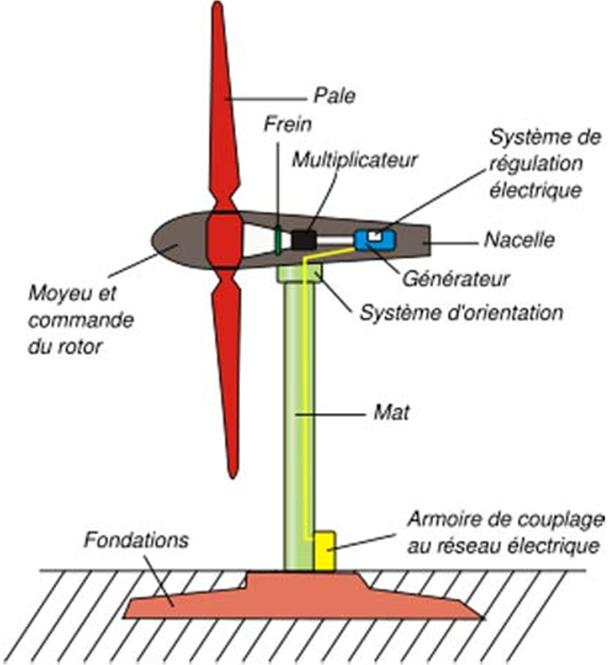
\includegraphics[scale=0.425]{img/eolienneTerrestre.png}
	\caption{\textup{Représentation schématique d’une éolienne terrestre.}}
    \label{eolienneTerrestre}
\end{figure}
\newpage


Les tableaux doivent être mis en forme avec le style défini dans le document modèle au format Word. Ils doivent être numérotés et légendés.
\begin{table}[!h]
    \centering	
    \caption{\textup{Liste des styles disponibles dans le modèle de rapport de stage au format Word}}
	\begin{tabular}{ll}
	    Nom         & Description                                   \\ \hline \hline
        Titre 1     & Titre du rapport                              \\ \hline
        Auteur      & Auteurs du rapport                            \\ \hline
        Institution & Institutions d’accueil du stage               \\ \hline
        Courriel	& Adresse électronique                          \\ \hline
        Titre 2	    & Titre de section sans numéro                  \\ \hline
        Titre 3	    & Titre de section avec numéro                  \\ \hline
        Mots-clefs	& Mots-clefs représentatifs du contenu du stage \\ \hline
        Normal	    & Texte du rapport                              \\ \hline
        Légendes	& Légendes des figures et tableaux              \\ \hline
	\end{tabular}
    \label{tableau1}
\end{table}


Les équations et les formules doivent être mise en forme avec un outil informatique adapté (éditeur d’équations) et doivent être numérotées :  
\begin{eqnarray}
   x & = & \frac{-b\pm \sqrt{b^2-4ac}}{2a}
\end{eqnarray}


Les références bibliographiques doivent être référencées\cite{ensicaenURL} dans le corps du texte par une numérotation et doivent être listées à la fin du rapport. La mise en forme des références bibliographiques varie en fonction de la nature de la référence citée. La référence \cite{troisiemeCentenaireNewton} illustre un article scientifique, les exemples [1] et \cite{wordURL} illustrent un lien internet,  et la référence \cite{theLatexCompanion} illustre un livre.

\subsubsection{Titre 4 : police calibri – taille 11 – noir simple italique}
Texte calibri – noir 11


\section{Le projet One Wave: Une carte universelle connectée}

\section{Introduction à la Tokenisation}
\subsection{Définition d'un Token}
\subsection{Pourquoi les Token?}

\section{Planning}


% Chapitre II :
\chapter{Etude de la spécification EMVCo "Payment Tokenisation Specification", 2014}

\section{Token Service Provider et Token Requestor}
\subsection{Token Service Provider}
\subsection{Token Requestor}

\section{Les Data elements}

\section{Demande et émission de Token}
\subsection{Les méthodes d'Identification et Vérification}
\subsection{Les interfaces: Token Service Provider APIs}

\section{Transaction EMV avec Token}
\subsection{Côté client - commerçant}
\subsection{Côté commerçant - autres acteurs de la transaction}

\section{Acquisition, compensation, règlement}
\subsection{Acquisition et compensation}
\subsection{Règlement}



% Bibliographie :
\renewcommand\bibname{\underline{Références bibliographiques}}
\bibliographystyle{unsrt}
\bibliography{biblio}
\newpage


% Couverture :
{\color{titre1}{\fontsize{16}{16} \selectfont {* Sur la dernière page (couverture) : \\ \\ \\
Résumé en français et en anglais avec mots clefs.}}}


\end{document}